% Round 2 findings section

\subsection{Round 2}

\subsubsection{Performance}

%%%
% Discussion of performance
%%%

% Point spreads for two runs of blah

\begin{figure}
\center

\begin{subfigure}[b]{0.45\textwidth}
	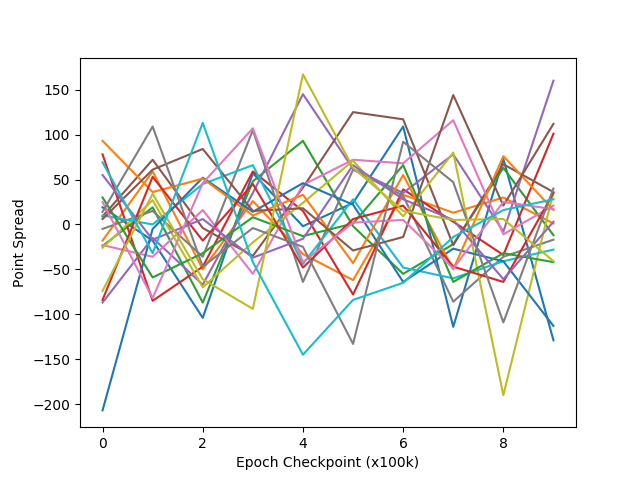
\includegraphics[width=\linewidth]{images/findings/round2/spreads_self-v-prev_winner.png}
	\caption{An agent plays against previous iterations of itself.}
	\label{fig:r2-spreads-winner-a}
\end{subfigure}
~
\begin{subfigure}[b]{0.45\textwidth}
	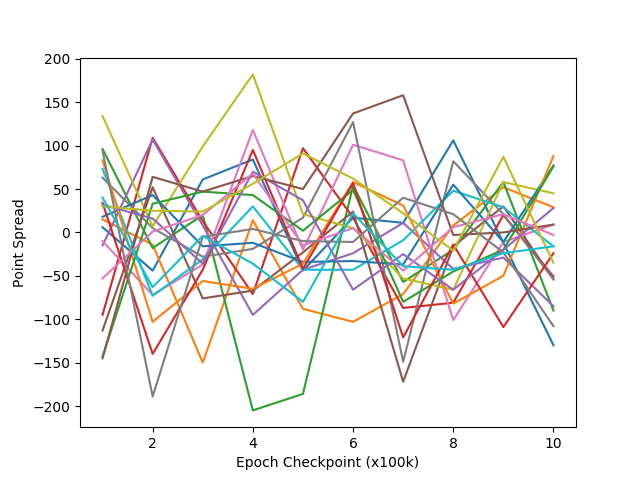
\includegraphics[width=\linewidth]{images/findings/round2/spreads_rand-v-fut_winner.png}
	\caption{A random agent plays against later, more learned agents.}
	\label{fig:r2-spreads-winner-b}
\end{subfigure}

\caption{
	Point spreads across twenty 9-game tournaments for an agent in the
	winners' bracket of Round 2.
	Note that since the winners' bracket uses an agent with prior training,
	the total epochs elapsed is one million more than displayed.
}
\label{fig:r2-spreads-winner}
\end{figure}


% Point spreads for two runs of blah

\begin{figure}
\center

\begin{subfigure}[b]{0.45\textwidth}
	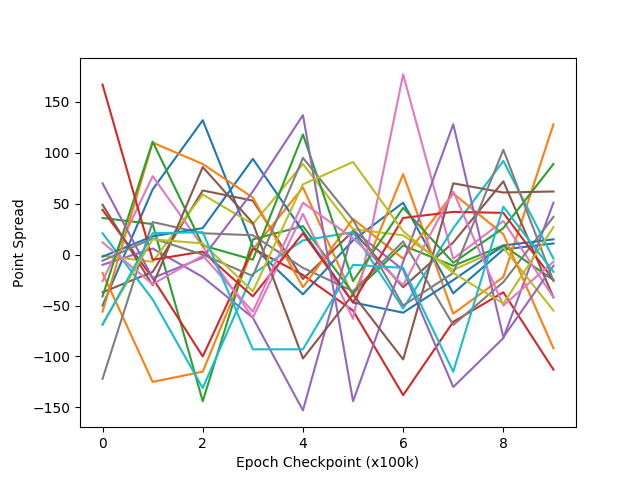
\includegraphics[width=\linewidth]{images/findings/round2/spreads_self-v-prev_loser.png}
	\caption{An agent plays against previous iterations of itself.}
	\label{fig:r2-spreads-loser-a}
\end{subfigure}
~
\begin{subfigure}[b]{0.45\textwidth}
	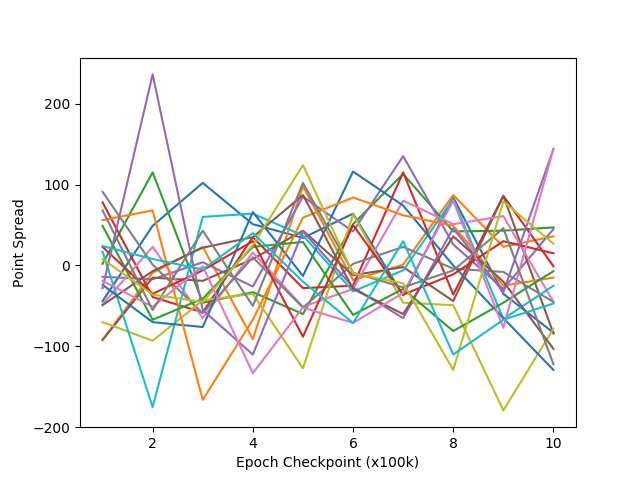
\includegraphics[width=\linewidth]{images/findings/round2/spreads_rand-v-fut_loser.png}
	\caption{A random agent plays against later, more learned agents.}
	\label{fig:r2-spreads-loser-b}
\end{subfigure}

\caption{
	Point spreads across mutliple 9-game tournamens of an agent in the
	losers' bracket of Round 2.
}
\label{fig:r2-spreads-loser}
\end{figure}




\subsubsection{Learning Process and Results}

%%%
% Discussion of what it learns and why that's interesting from a cribbage
% perspective
%%%

%%%
Despite the lack of performance increase after another million games played by
both the winning and losing brackets,
there are still interesting trends to be spotted between the different brackets
of play.
%
The most notable is how quickly policies converge to a similar state.
%
While the strategy graphs for the less trained agents are less ``crisp''
in their appearance thanks to their smaller levels self-certainty,
the patterns of which policy to mainly follow at which times
are quick to form.
%
This is useful because it allows for the possibility of running future
experiments with fewer training epochs and thus in less time.
%
This in turn allows for a larger variety of methods to be tested to improve
the cribbage-playing agent.
%%%

%%%
Even more fascinating observations can be found from the strategy graphs
from the winner's bracket (see Figure~\ref{r2-strats-winner}).
%
By focusing on the \handmaxmin\ and \handmaxavg\ strategies in particular,
the sinusoidal wave along the diagonal can be observed extending further
back along the diagonal to earlygame positions.
%
While not being of much use to the agent directly,
this is a useful observation for a 
% TODO: continue
%%%

% Figure for the flipbook of strategies over time

\begin{figure}
\center

	\begin{subfigure}[b]{0.4\textwidth}
	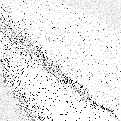
\includegraphics[width=\linewidth]{images/findings/round2/flipbook/winner/checkpoint_000000.png}
	\caption{Starting Weights}
	\end{subfigure}
	~
	\begin{subfigure}[b]{0.4\textwidth}
	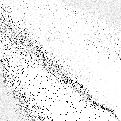
\includegraphics[width=\linewidth]{images/findings/round2/flipbook/winner/checkpoint_200000.png}
	\caption{After 200,000 games played}
	\end{subfigure}

	\begin{subfigure}[b]{0.4\textwidth}
	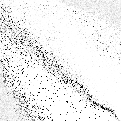
\includegraphics[width=\linewidth]{images/findings/round2/flipbook/winner/checkpoint_400000.png}
	\caption{After 400,000 games played}
	\end{subfigure}
	~
	\begin{subfigure}[b]{0.4\textwidth}
	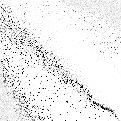
\includegraphics[width=\linewidth]{images/findings/round2/flipbook/winner/checkpoint_600000.png}
	\caption{After 600,000 games played}
	\end{subfigure}

	\begin{subfigure}[b]{0.4\textwidth}
	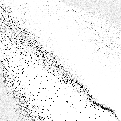
\includegraphics[width=\linewidth]{images/findings/round2/flipbook/winner/checkpoint_800000.png}
	\caption{After 800,000 games played}
	\end{subfigure}
	~
	\begin{subfigure}[b]{0.4\textwidth}
	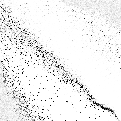
\includegraphics[width=\linewidth]{images/findings/round2/flipbook/winner/checkpoint_999999.png}
	\caption{Final Weights}
	\end{subfigure}

\caption{
	Training weights representation for a winner bracket agent's \handmaxavg\
	strategy when the agent is the dealer
	over the course of the one million games of Round 2.
	Note that the starting weights are carried over from Round 1,
	so the total training epochs to reach each position is actually
	one million higher than expressed.
}
\label{fig:r2-flip-winner}
\end{figure}


% Figure for the flipbook of strategies over time

\begin{figure}
\center

	\begin{subfigure}[t]{0.2\textwidth}
	
\includegraphics[width=\textwidth]{images/findings/round2/flipbook/loser/checkpoint_000000.png}
	\caption{Starting Weights}
	\end{subfigure}
	~
	\begin{subfigure}[t]{0.2\textwidth}
	\includegraphics[width=\textwidth]{images/findings/round2/flipbook/loser/checkpoint_200000.png}
	\caption{After 200,000 games played}
	\end{subfigure}
	~
	\begin{subfigure}[t]{0.2\textwidth}
	\includegraphics[width=\textwidth]{images/findings/round2/flipbook/loser/checkpoint_400000.png}
	\caption{After 400,000 games played}
	\end{subfigure}

	\begin{subfigure}[t]{0.2\textwidth}
	\includegraphics[width=\textwidth]{images/findings/round2/flipbook/loser/checkpoint_600000.png}
	\caption{After 600,000 games played}
	\end{subfigure}
	~
	\begin{subfigure}[t]{0.2\textwidth}
	\includegraphics[width=\textwidth]{images/findings/round2/flipbook/loser/checkpoint_800000.png}
	\caption{After 800,000 games played}
	\end{subfigure}
	~
	\begin{subfigure}[t]{0.2\textwidth}
	\includegraphics[width=\textwidth]{images/findings/round2/flipbook/loser/checkpoint_999999.png}
	\caption{Final Weights}
	\end{subfigure}

\caption{
	Training weights representation for a losers' bracket agent's \handmaxavg\
	strategy when the agent is the dealer
	over the course of the one million games of Round 2.
}
\label{fig:r2-flip-loser}
\end{figure}


% Figure for the flipbook of strategies over time

\begin{figure}
\center

	\begin{subfigure}[b]{0.4\textwidth}
	
\includegraphics[width=\linewidth]{images/findings/round2/flipbook/random/checkpoint_000000.png}
	\caption{Starting Weights}
	\end{subfigure}
	~
	\begin{subfigure}[b]{0.4\textwidth}
	\includegraphics[width=\linewidth]{images/findings/round2/flipbook/random/checkpoint_200000.png}
	\caption{After 200,000 games played}
	\end{subfigure}

	\begin{subfigure}[b]{0.4\textwidth}
	\includegraphics[width=\linewidth]{images/findings/round2/flipbook/random/checkpoint_400000.png}
	\caption{After 400,000 games played}
	\end{subfigure}
	~
	\begin{subfigure}[b]{0.4\textwidth}
	\includegraphics[width=\linewidth]{images/findings/round2/flipbook/random/checkpoint_600000.png}
	\caption{After 600,000 games played}
	\end{subfigure}

	\begin{subfigure}[b]{0.4\textwidth}
	\includegraphics[width=\linewidth]{images/findings/round2/flipbook/random/checkpoint_800000.png}
	\caption{After 800,000 games played}
	\end{subfigure}
	~
	\begin{subfigure}[b]{0.4\textwidth}
	\includegraphics[width=\linewidth]{images/findings/round2/flipbook/random/checkpoint_999999.png}
	\caption{Final Weights}
	\end{subfigure}

\caption{
	Training weights representation for a winner bracket agent's \handmaxavg\
	strategy when the agent is the dealer
	over the course of the one million games of Round 2.
}
\label{fig:r2-flip-random}
\end{figure}



\begin{figure}
\center

	\begin{subfigure}[t]{0.22\textwidth}
		
\includegraphics[width=\textwidth]{images/findings/round2/strats/winner/hand_max_min.png}
		\caption{\handmaxmin}
	\end{subfigure}
	~
	\begin{subfigure}[t]{0.22\textwidth}
		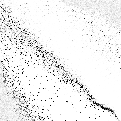
\includegraphics[width=\textwidth]{images/findings/round2/strats/winner/hand_max_avg.png}
		\caption{\handmaxavg}
	\end{subfigure}
	~
	\begin{subfigure}[t]{0.22\textwidth}
		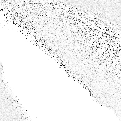
\includegraphics[width=\textwidth]{images/findings/round2/strats/winner/hand_max_med.png}
		\caption{\handmaxmed}
	\end{subfigure}
	~
	\begin{subfigure}[t]{0.22\textwidth}
		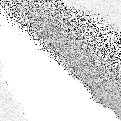
\includegraphics[width=\textwidth]{images/findings/round2/strats/winner/hand_max_poss.png}
		\caption{\handmaxposs}
	\end{subfigure}

	\begin{subfigure}[t]{0.22\textwidth}
		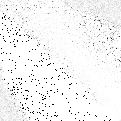
\includegraphics[width=\textwidth]{images/findings/round2/strats/winner/crib_min_avg.png}
		\caption{\cribminavg}
	\end{subfigure}
	~
	\begin{subfigure}[t]{0.22\textwidth}
		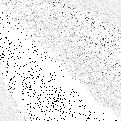
\includegraphics[width=\textwidth]{images/findings/round2/strats/winner/pegging_max_avg_gained.png}
		\caption{\peggingmaxavggained}
	\end{subfigure}
	~
	\begin{subfigure}[t]{0.22\textwidth}
		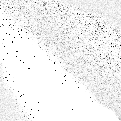
\includegraphics[width=\textwidth]{images/findings/round2/strats/winner/pegging_max_med_gained.png}
		\caption{\peggingmaxmedgained}
	\end{subfigure}
	~
	\begin{subfigure}[t]{0.22\textwidth}
		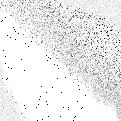
\includegraphics[width=\textwidth]{images/findings/round2/strats/winner/pegging_min_avg_given.png}
		\caption{\peggingminavggiven}
	\end{subfigure}

\caption{
	All final strategy strengths for an agent in the winners' bracket
	when playing as the dealer
	after training for one million games during Round 1
	and a further one million games during Round 2.
}
\label{fig:r2-strats-winner}
\end{figure}



\begin{figure}
\center

	\begin{subfigure}[t]{0.22\textwidth}
		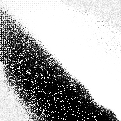
\includegraphics[width=\stratgraphwidth]{images/findings/round2/strats/loser/hand_max_min.png}
		\caption{\handmaxmin}
	\end{subfigure}
	~
	\begin{subfigure}[t]{0.22\textwidth}
		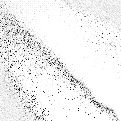
\includegraphics[width=\stratgraphwidth]{images/findings/round2/strats/loser/hand_max_avg.png}
		\caption{\handmaxavg}
	\end{subfigure}
	~
	\begin{subfigure}[t]{0.22\textwidth}
		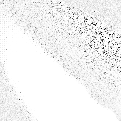
\includegraphics[width=\stratgraphwidth]{images/findings/round2/strats/loser/hand_max_med.png}
		\caption{\handmaxmed}
	\end{subfigure}
	~
	\begin{subfigure}[t]{0.22\textwidth}
		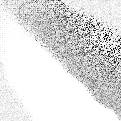
\includegraphics[width=\stratgraphwidth]{images/findings/round2/strats/loser/hand_max_poss.png}
		\caption{\handmaxposs}
	\end{subfigure}

	\begin{subfigure}[t]{0.22\textwidth}
		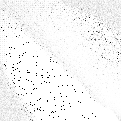
\includegraphics[width=\stratgraphwidth]{images/findings/round2/strats/loser/crib_min_avg.png}
		\caption{\cribminavg}
	\end{subfigure}
	~
	\begin{subfigure}[t]{0.22\textwidth}
		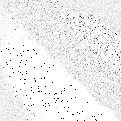
\includegraphics[width=\stratgraphwidth]{images/findings/round2/strats/loser/pegging_max_avg_gained.png}
		\caption{\peggingmaxavggained}
	\end{subfigure}
	~
	\begin{subfigure}[t]{0.22\textwidth}
		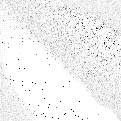
\includegraphics[width=\stratgraphwidth]{images/findings/round2/strats/loser/pegging_max_med_gained.png}
		\caption{\peggingmaxmedgained}
	\end{subfigure}
	~
	\begin{subfigure}[t]{0.22\textwidth}
		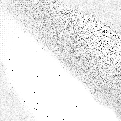
\includegraphics[width=\stratgraphwidth]{images/findings/round2/strats/loser/pegging_min_avg_given.png}
		\caption{\peggingminavggiven}
	\end{subfigure}

\caption{
	All final strategy strengths for an agent in the losers' bracket
	when playing as the dealer
	after training for one million games during Round 2.
}
\label{fig:r2-strats-loser}
\end{figure}



\begin{figure}
\center

	\begin{subfigure}[t]{0.22\textwidth}
		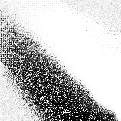
\includegraphics[width=\stratgraphwidth]{images/findings/round2/strats/random/hand_max_min.png}
		\caption{\handmaxmin}
	\end{subfigure}
	~
	\begin{subfigure}[t]{0.22\textwidth}
		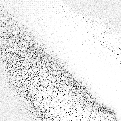
\includegraphics[width=\stratgraphwidth]{images/findings/round2/strats/random/hand_max_avg.png}
		\caption{\handmaxavg}
	\end{subfigure}
	~
	\begin{subfigure}[t]{0.22\textwidth}
		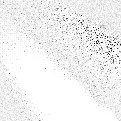
\includegraphics[width=\stratgraphwidth]{images/findings/round2/strats/random/hand_max_med.png}
		\caption{\handmaxmed}
	\end{subfigure}
	~
	\begin{subfigure}[t]{0.22\textwidth}
		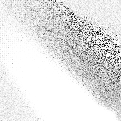
\includegraphics[width=\stratgraphwidth]{images/findings/round2/strats/random/hand_max_poss.png}
		\caption{\handmaxposs}
	\end{subfigure}

	\begin{subfigure}[t]{0.22\textwidth}
		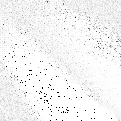
\includegraphics[width=\stratgraphwidth]{images/findings/round2/strats/random/crib_min_avg.png}
		\caption{\cribminavg}
	\end{subfigure}
	~
	\begin{subfigure}[t]{0.22\textwidth}
		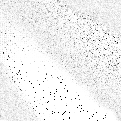
\includegraphics[width=\stratgraphwidth]{images/findings/round2/strats/random/pegging_max_avg_gained.png}
		\caption{\peggingmaxavggained}
	\end{subfigure}
	~
	\begin{subfigure}[t]{0.22\textwidth}
		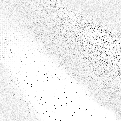
\includegraphics[width=\stratgraphwidth]{images/findings/round2/strats/random/pegging_max_med_gained.png}
		\caption{\peggingmaxmedgained}
	\end{subfigure}
	~
	\begin{subfigure}[t]{0.22\textwidth}
		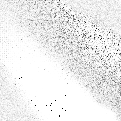
\includegraphics[width=\stratgraphwidth]{images/findings/round2/strats/random/pegging_min_avg_given.png}
		\caption{\peggingminavggiven}
	\end{subfigure}

\caption{
	All final strategy strengths for a learning agent
	after playing a completely random agent
	when playing as the pone
	after training for 350,000 games during Round 2.
}
\label{fig:r2-strats-random}
\end{figure}


